\documentclass[11pt]{article}

\usepackage{amsmath}
\usepackage{amssymb} 
\usepackage{textcomp}
\usepackage{float}
\usepackage[top=0.8in, bottom=0.8in, left=0.8in, right=0.8in]{geometry}
\usepackage{graphicx}
\usepackage{wrapfig}
\graphicspath{ {./} }
% Add other packages here %


% put your group number and names in the author field
\title{\bf Exercise 2: A Reactive Agent for the Pickup and Delivery Problem}
\author{Group \textnumero: 90  Kyle Gerard, Yann Bolliger}

% the report should not be longer than 3 pages

\begin{document}
\maketitle

\section{Problem Representation}

\subsection{Representation Description}

We wanted our state to contain two types of information: the current city of the 
agent as well as the fact whether there is a task available in this city. For 
the tasks, we also need to distinguish between the different destinations of the 
tasks. Therefore our state is modelled by a tuple from the set:
$$
\mathcal{S} = \{ (c_{curr}, c_{dest})  \, | \, 
c_{curr} \in \mathcal{C},  
c_{dest} \in (\mathcal{C} - \{ c_{curr}\}) \cup \{\mathtt{null}\} }
 \}
$$
where $\mathcal{C}$ is the set of all cities. Note that $\mathtt{null}$ denotes 
the case where there is no task available in the current city.
The exclusion of $c_{curr}$ in the second place encodes that there are no 
tasks with delivery city equal to the pickup city.

Our actions are either a \texttt{Pickup} for the given task or a \texttt{Move} to a 
neighboring city given by the set:
$$
\mathcal{A} = \{ \mathtt{Pickup} \} \cup \{ \mathtt{Move}(c)  \, | \,  c \in \mathcal{C} \}
$$

Given this representation of the problem the reward table $R(s, a)$ is defined in 
straight-forward way. It is the expected reward 
the agent gets for a delivery $r(c_i, c_j)$ minus the cost
for the travelled distance:
$$
R(s = (c_i, c_j) , a) = \begin{cases}
r(c_i, c_j) - k  \cdot d(c_i, c_j) , &  \text{if } a = \mathtt{Pickup} \\
- k  \cdot d(c_i, c_{neighbor}) , & \text{if } a = \mathtt{Move}(c_{neighbor}) 
\end{cases}
$$
where $d()$ is the function that calculates the optimal distances and $k$ is the cost 
per kilometer of the vehicle. 

In order to explain the transition table $T(s, a, s')$ we have to think about 
what it means to go from a state $(c_i, c_j)$ to a state $(c_n, c_m)$. It is 
important to note that  $T(s, a, s') = \mathbb{P}(s' | s, a)$; the action that 
the agent takes is given. 
 
 \begin{enumerate}
   
\item 
If the agent does \texttt{Move},  
he ends up in state $(c_n, c_m)$ if $c_n$ is a neighbor of $c_i$ and if there is 
a task to city $c_m$ (or \texttt{null}) in $c_n$.
This happens with the probability  given by the provided distribution $p(c_n, c_m)$.

\item If the agent does \texttt{Pickup},  
he ends up in state $(c_n, c_m)$ if $c_n$ is the destination of the task and if there is 
a task to city $c_m$ (or \texttt{null}) in $c_n$.
This happens also with the probability $p(c_n, c_m)$.

\item 
In all other cases the transition is impossible, therefore $T(s, a, s') = 0$. 
This can happen if the action is \texttt{Pickup} but there is no task or if the 
end and start cities are not the same or not neighbors.

\end{enumerate}



\subsection{Implementation Details}
For our states and actions, we created two specific classes to model 
them exactly as described above: \texttt{State, ActionSpaceElem}.
Additionally, there are two methods that return the state space $\mathcal{S}$ and the set of 
actions $\mathcal{A}$. This allows us to loop naturally over the entire 
spaces like in the theoretical pseudo-code for value iteration 
(e.g. $\forall s \in \mathcal{S}$ \texttt{do ...}). 

However, in order to avoid bugs in the extreme case where $\gamma = 0$ 
and in order to be faster, we filter the actions that are used in the loop 
based on the current state of the outer loop. This is done by the 
method \texttt{getPossibleActions}. The method filters for 
example all \texttt{Move} actions that lead to non-neighboring cities. Or when
 $\gamma = 0$, it prevents the agent from wanting to move to the city 
where it currently is.

The value iteration algorithm stops when the approximation of $V(s)$ is ``good 
enough''.
We chose to calculate the mean square error between the $V(s)$ of two 
consecutive iterations and to stop the algorithm when the error was $ < 
\epsilon = 10^{-16}$. This corresponds to approximately 200 iterations for
the french map and we found that an $\epsilon < 10^{-16}$ didn't provide any 
advantage because the strategy $Best(s)$ usually converges much faster.


Finally, our $V(s)$ and $Best(s)$ are implemented using \texttt{HashMap}s for 
optimal performance. We provided the \texttt{State} class with an appropriate 
hash-function. In the \texttt{act} function it is therefore sufficient to instantiate 
the state based on the arguments of the function and to retrieve the best action 
from the latest $Best(s)$. This happens in $\mathcal{O}(1)$ time thanks to the 
\texttt{HashMap}.


\section{Results}
% in this section, you describe several results from the experiments with your reactive agent

\subsection{Experiment 1: Discount factor}
% the purpose of this experiment is to understand how the discount factor influences the result

\subsubsection{Setting}
% you describe how you perform the experiment (you also need to specify the configuration used for the experiment)
 \begin{table}[H]
  \begin{tabular}{llll}
   &\texttt{map }  &Netherlands / France\\
   &\texttt{config}  & given config files reactive2.xml and reactive.xml \\
   &\texttt{agent}  &reactive-rla\\
   &\texttt{discount factor}  &$x$ between [0, 1[\\
   &\texttt{steps}  &2000
  \end{tabular}
 \end{table}

\subsubsection{Observations}
% you describe the experimental results and the conclusions you inferred from these results

\subsection{Experiment 2: Comparisons with dummy agents}
% you compare the results of your agent with two dummy agents: the random agent that was already given in the starter files and another dummy agent that you define and create. You should report the results from the simulations using the topologies given in the starter files and optionally, additional topologies that you create.
 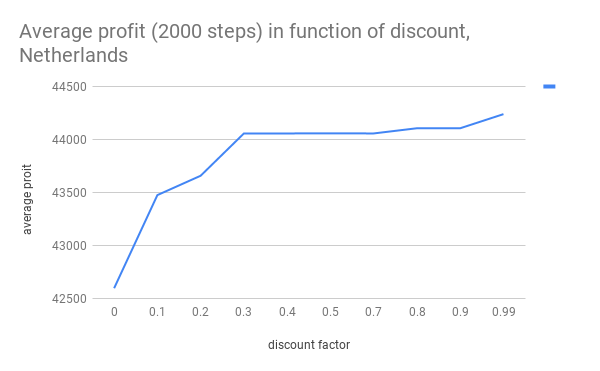
\includegraphics[width=0.5\textwidth]{netherlands.png}
 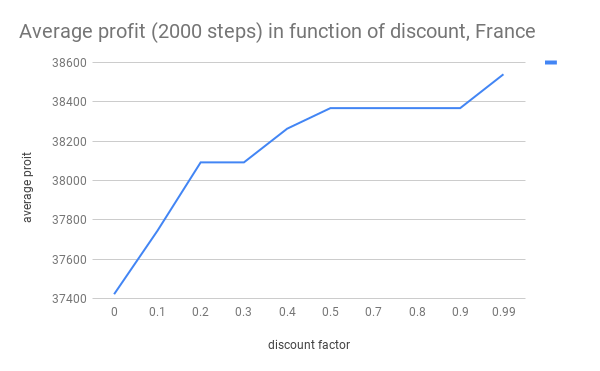
\includegraphics[width=0.5\textwidth]{france.png}
In this experiment we examine how the discount factor influences the behavior of the agent and thus its profit. As seen in both of the above graphs, with these settings, higher discount factors lead to higher average profits per action (and consequently higher total profits) with a large number of steps. This makes sense as a high discount factor encourages the agent to take good long term decisions by giving more importance to the values of the future states it might travel to. With a low discount factor, short term rewards are prioritized. The reason why the lowest average profit is with a 0 discount factor is because this means the agent is completely blind to the values of the states around him and thus moves randomly to a neighboring city when there is no task in a city. 

However, a lower discount factor does not always mean a lower profit depending on how many steps the simulation lasts. Indeed, during our first version of this experiment we only used 200 steps to compare the average profits of different discount values. However, as the tasks and rewards are generated randomly, we observed that the highest profits were between 0.6 and 0.7 discount values. This randomness means that even though an agent has the best policy, it may not have the best profit after a given finite number of steps.
Finally, we observe that with a higher discount factor, the learning phase lasts more iterations and converges more slowly. In the extreme case with a discount factor of 1, it does not converge.

\subsubsection{Setting}
% you describe how you perform the experiment and you describe the dummy agent you created (you also need to specify the configuration used for the experiment)
 \begin{table}[H]
  \begin{tabular}{llll}
   &\texttt{map }  &Netherlands / France\\
   &\texttt{config}  & given config files reactive2.xml and reactive.xml \\
   &\texttt{agent}  &reactive-rla reactive-dummy reactive-random\\
   &\texttt{discount factor}  &0.6\\
   &\texttt{steps}  &2000
  \end{tabular}
 \end{table}
 
 The reactive-random agent uses random Move decisions and a pickup probability = 0.6 when a task is available.
The reactive-Dummy agent has a 100 percent pickup probability and always moves to closest neighboring City.

 
\subsubsection{Observations}
% elaborate on the observed results
 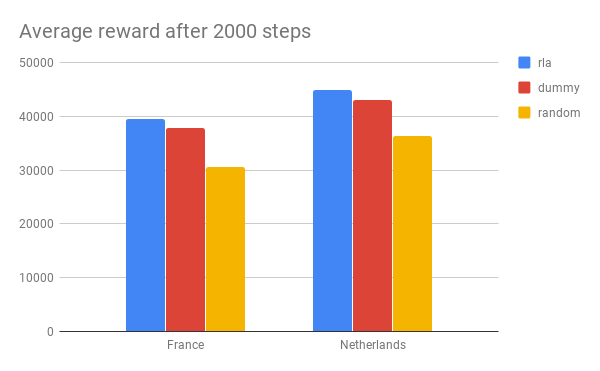
\includegraphics[width=0.6\textwidth]{agents.png}

In the above bar chart we observe that the best performing agent is the smart rla agent and the worst is the random agent. The reason why the random agent is so much worse than the other agents with both topologies is mainly because it does not pickup a large proportion of tasks (40 percent).

We also remark that the rla agent and the Dummy agent’s average profits are relatively close. By observing the rla agent’s policy we see that it almost always picks up a task when one is available (as opposed to Moving to a neighboring city instead). This means that the only difference between the two agents is the slight advantage the rla agent has in choosing which city to move to when no task is available (because it knows which neighboring city has the most value).


\end{document}
